\documentclass[border=8pt]{standalone}
\usepackage{pgfplots}
\pgfplotsset{compat=1.18}
\begin{document}
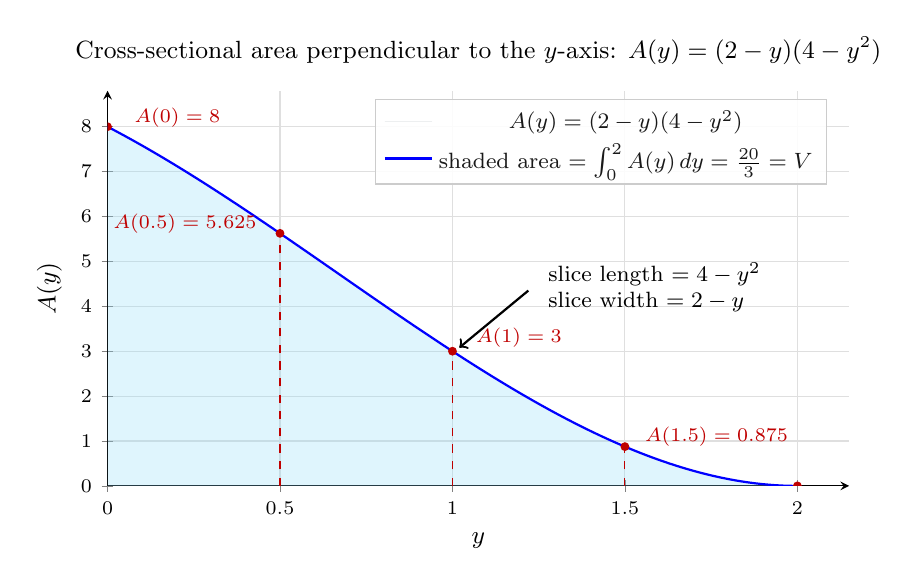
\begin{tikzpicture}
\begin{axis}[
    width=11cm, height=6.6cm,
    xlabel={$y$}, ylabel={$A(y)$},
    xmin=0, xmax=2.15, ymin=0, ymax=8.8,
    xtick={0,0.5,1.0,1.5,2.0}, ytick={0,1,2,3,4,5,6,7,8},
    ticklabel style={font=\scriptsize},
    label style={font=\small},
    title={Cross-sectional area perpendicular to the $y$-axis: $A(y)=(2-y)(4-y^2)$},
    title style={font=\small},
    grid=major, grid style={gray!25},
    axis x line=left, axis y line=left,
    legend style={font=\footnotesize, at={(0.97,0.98)}, anchor=north east,
                  fill=white, fill opacity=0.9, draw=gray!40},
]
\addplot[fill=cyan!45, opacity=0.28, draw=none, domain=0:2, samples=200]
    ({x}, {(2-x)*(4-x^2)}) \closedcycle;
\addplot[thick, blue, domain=0:2, samples=200, mark=none] ({x}, {(2-x)*(4-x^2)});
\addlegendentry{$A(y)=(2-y)(4-y^2)$}
\addlegendimage{empty legend}
\addlegendentry{shaded area $=\int_0^2 A(y)\,dy=\frac{20}{3}=V$}

\draw[red!75!black, dashed, thin] (axis cs:0.5,0) -- (axis cs:0.5,5.625);
\draw[red!75!black, dashed, thin] (axis cs:1.0,0) -- (axis cs:1.0,3);
\draw[red!75!black, dashed, thin] (axis cs:1.5,0) -- (axis cs:1.5,0.875);
\fill[red!75!black] (axis cs:0,8) circle (1.6pt);
\fill[red!75!black] (axis cs:0.5,5.625) circle (1.6pt);
\fill[red!75!black] (axis cs:1.0,3) circle (1.6pt);
\fill[red!75!black] (axis cs:1.5,0.875) circle (1.6pt);
\fill[red!75!black] (axis cs:2.0,0) circle (1.6pt);

\node[font=\scriptsize, red!75!black, anchor=west] at (axis cs:0.05,8.20) {$A(0)=8$};
\node[font=\scriptsize, red!75!black, anchor=east] at (axis cs:0.46,5.85) {$A(0.5)=5.625$};
\node[font=\scriptsize, red!75!black, anchor=west] at (axis cs:1.04,3.30) {$A(1)=3$};
\node[font=\scriptsize, red!75!black, anchor=west] at (axis cs:1.53,1.10) {$A(1.5)=0.875$};
\node[font=\scriptsize, red!75!black, anchor=north east] at (axis cs:1.98,0.02) {$A(2)=0$};

\draw[->, thick] (axis cs:1.22,4.35) -- (axis cs:1.02,3.08);
\node[font=\footnotesize, align=left, anchor=west] at (axis cs:1.25,4.42)
     {slice length $=4-y^2$\\ slice width $=2-y$};
\end{axis}
\end{tikzpicture}
\end{document}